\documentclass{article}
\usepackage[utf8x]{inputenc}
\usepackage[T1, T2A]{fontenc}
\usepackage[russian]{babel}
\usepackage{amsmath}
\usepackage{graphicx} 
\usepackage{amssymb}
\setlength\parindent{0pt}
\usepackage[parfill]{parskip}
\pagenumbering{gobble}

\begin{document}
Рассмотрим несколько случаев:\\
1) $x<1$. Тогда $x^n$ и $( \frac{x^2}{2} )^n$ стремятся к нулю при $n \to \infty$ и, следовательно,
$$\lim\limits_{n\to \infty} \sqrt[n]{1 + x^n + \left( \frac{x^2}{2} \right)^n} = 1.$$
2) $1 \leqslant x < 2$. Тогда $\frac{x}{2} < 1$ и мы имеем
$$\sqrt[n]{1 + x^n + \left( \frac{x^2}{2} \right)^n} = x \sqrt[n]{\frac{1}{x^n} + 1 + \left( \frac{x}{2} \right)^n} \to x\;\;(n \to \infty).$$
3) $x \geqslant 2$. Тогда $\frac{2}{x} \leqslant 1$ и мы имеем
$$\sqrt[n]{1 + x^n + \left( \frac{x^2}{2} \right)^n} = \frac{x^2}{2} \sqrt[n]{\left( \frac{2}{x^2} \right)^n + \left( \frac{2}{x} \right)^n + 1} \to \frac{x^2}{2}\;\;(n \to \infty).$$
Получается следующий график (правый участок графика представляет собою часть параболы):
\begin{figure}[h]
\center{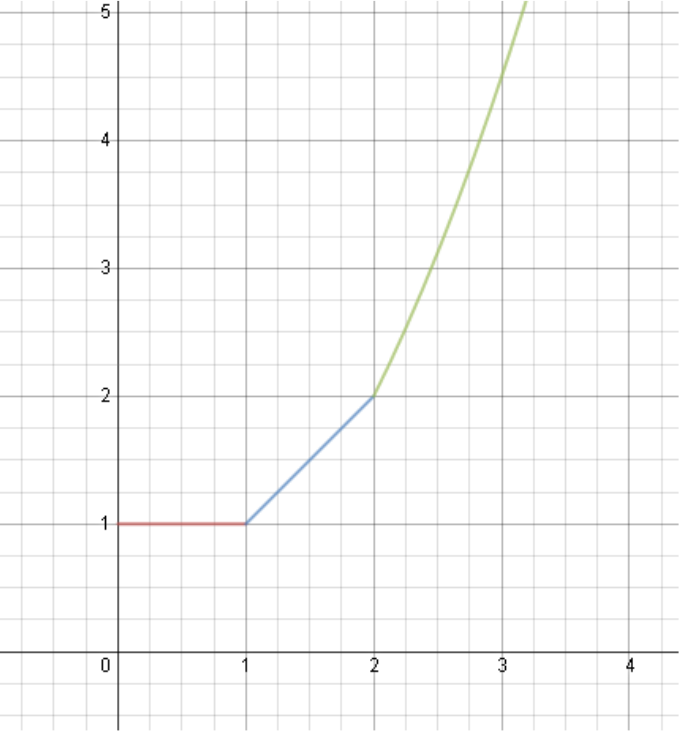
\includegraphics[width=0.6\textwidth]{graph}}
\end{figure}
\end{document}
